\chapter{Apprendre des demandes de crédit à la consommation} \label{chap1}

Ce chapitre est destiné à poser les bases de l'apprentissage statistique dans le cadre des crédits à la consommation. On introduira dans une première partie une partie de la terminologie consacrée aux crédits à la consommation avant de s'attarder plus en détails, dans une seconde partie, sur l'état de l'art industriel du \textit{Credit Scoring} à travers une étude bibliographique et la pratique de \gls{cacf}. On clotûrera le chapitre par une troisième partie, la plus traditionnelle pour débuter un manuscrit de thèse, à savoir l'état de l'art académique sur l'apprentissage statistique, en nous limitant bien entendu aux cas d'usage spécifiques aux crédits à la consommation mis en exergue dans les deux premières parties de ce chapitre.

\section{Le marché du crédit à la consommation : quels enjeux ?} \label{chap1:sec1}

S'agissant d'une thèse CIFRE, il apparaît comme nécessaire de planter le décor industriel de la problématique. Dans cette première partie, on verra succintement le coeur du métier de \gls{cacf}, les produits qu'elles proprosent et l'environnement dans lequel elle s'insert.

\subsection{Qu'est-ce qu'un crédit à la consommation ?}

La définition légale en a été donnée en~\ref{chap_intro}. En pratique, on peut distinguer trois produits de crédit à la consommation.


Le premier d'entre eux, le \gls{creditclassique} est le produit historique. De la même manière qu'un crédit immobilier, le client emprunte une somme fixe qui lui est attribuée au financement et qu'il rembourse selon un échéancier (taux et nombre de mensualités fixes) défini à l'avance. D'un point de vue statistique, le traitement est relativement simple : que ce soit à l'octroi, pour déterminer le risque du client, ou au cours de la vie du dossier, pour provisionner les pertes potentielles, tout est connu à l'avance. Il suffit en quelque sorte de vérifier le paiement de la mensualité à la date prévue. Il convient également de préciser que certains crédits classiques sont dits \glspl{creditaffecte}, c'est-à-dire qu'ils financent un bien précis et identifié, de sorte que le prêt transite directement de l'organisme prêteur au vendeur (concessionnaire par exemple). Par ailleurs, la mise en défaut du crédit entraîne généralement une procédure de recouvrement de la dette qui peut se solder, dans le cas d'un \gls{creditaffecte}, par la récupération du bien par un huissier. Là encore, d'un point de vue statistique, il paraît indispensable de consigner les caractéristiques du bien sous-jacent afin d'intégrer sa valeur résiduelle récupérable en cas de défaut.


Le second produit, développé à partir de 1965 en France et ayant connu une forte croissance depuis~\cite{ducourant2009credit} mais néanmoins bien moins répandu en Europe qu'aux Etats-Unis par exemple~\cite{credit_cards_country}, est le \gls{creditrenouvelable}. Un capital dit accordé ou autorisé est attribué au demandeur qui peut utiliser tout ou partie de ce montant et le rembourse à un taux et par mensualités dépendants tous deux de la proportion du capital consommé. Au fur et à mesure du remboursement du capital emprunté, le capital ‘‘empruntable'', c'est-à-dire la différence entre le capital accordé et le capital emprunté puis remboursé, se reconstitue et de nouvelles utilisations sont possibles, toujours dans la limite du capital accordé au départ. D'un point de vue statistique à nouveau, plusieurs problèmes se posent du fait du caractère intrinsèquement aléatoire de l'utilisation ou non de tout ou partie de la ligne de crédit accordée. Plus précisément, ce produit présente un risque important porté par deux facteurs : premièrement, le taux élevé attire des clients risqués, au taux de défaut plus élevé que pour un crédit classique par exemple ; deuxièmement, ces crédits portent un risque dit de hors-bilan très fort, puisqu'à tout moment, l'ensemble des crédits accordés mais non utilisés et donc non comptabilisés ‘‘au bilan'' c'est-à-dire comme une dette du client envers l'établissement bancaire, peuvent être utilisés et faire défaut. La mauvaise quantification de ce risque est à présent reconnu comme un important catalyseur de la récente crise financière \cite{karim2013off}.


Enfin, la \gls{location} a récemment connu un essor important~\cite{peden_2018}. D'abord concentrée sur le secteur automobile, elle se développe actuellement pour les produits électroniques (smartphones notamment) et même plus récemment pour des produits plus insolites comme les matelas~\cite{dicharry_2017}. Comme le \gls{creditaffecte}, il est important de prendre en compte les données du bien loué afin d'évaluer le risque que porte ce produit, la difficulté supplémentaire reposant sur l'éventualité de l'exercice de l'option d'achat.

De cette partie, deux considérations statistiques doivent retenir notre attention : d'abord, ces différents produits nécessitent des traitements différents dans la mesure où leur risque est intrinsèquement différent ; ensuite, les données disponibles pour chacun de ces produits diffèrent : par exemple, les données du produit financé ne sont disponibles que pour les \glspl{creditaffecte} et les \glspl{location}. Cette dernière notion de ‘‘blocs'' de variables est au coeur du chapitre~\ref{chap6}.

%\subsection{Quels sont les acteurs de ce marché ?}
%Au même titre que la partie précédente, cette partie ne se veut pas une analyse du marché du crédit à la consommation mais 

\subsection{Crédit Agricole Consumer Finance}

\gls{cacf} opère dans de nombreux pays. En France, c'est principalement à travers la marque Sofinco que sont commercialisés les crédits à la consommation pour lesquels il existe une relation directe entre \gls{cacf} et le client (dite B2C), par exemple lorsqu'un demandeur se rend directement sur le site internet \href{https://www.sofinco.fr}{sofinco.fr}.

Par ailleurs, de nombreux crédits à la consommation sont distribués à travers un réseau de partenaires, qui jouent le rôle d'intermédiaires (on parle alors de B2B) : concessionnaires automobile, distributeurs d'électroménager, etc.

Enfin, \gls{cacf} faisant partie du groupe Crédit Agricole, de nombreuses Caisses Régionales distribuent des crédits à la consommation à leur clientèle bancarisé, par l'intermédiaire des gestionnaires de compte.

Là encore, on constate que les spécificités des canaux de distribution des crédits impactent grandement la collecte des données et leur traitement statistique. En effet, les informations collectées sur le client, le produit et éventuellement l'apporteur d'affaires sont différentes selon le canal.

Dans la partie suivante, la méthodologie présentée est spécifique à \gls{cacf} ; il pourra néanmoins être admis que, dans les grandes lignes, cette méthodologie est similaire à la concurrence d'une part, et à la pratique d'autres pays (européens du moins) puisque la législation sur la protection et le traitement des données est sensiblement similaire (du fait de l'entrée en vigueur récente de la GDPR) et les établissements bancaires possèdent généralement des filiales dans plusieurs pays d'Europe et y font appliquer la même méthodologie.

% disclaimer
%Par ailleurs, les données réelles utilisées pour illustrer les méthodologies statistiques présentées dans ce manuscrit sont la propriété de \gls{cacf}.

\section{Le \textit{Credit Scoring} : état de l'art de la pratique industrielle} \label{chap1:sec2}

Cette partie vise à présenter la pratique actuelle en matière de \textit{Credit Scoring} et pose un certain nombre de questions statistiques dont certaines ont été traitées dans cette thèse, d'autres trouvent des réponses (parfois partielles) dans la litérature et dont certaines références sont données à titre informatif mais ne sont pas développées dans ce manuscrit ; enfin, certaines questions ne trouvent \textit{a priori} pas de réponse immédiate dans la litérature et sont autant de matière à de futurs travaux dans le domaine !

\subsection{Collecte des données}

La partie précédente a mis en exergue la pluralité des sources de données. La figure~\ref{fig:souscription} présente par exemple le formulaire de souscription en vigueur pour un crédit automobile auprès de Sofinco \textit{via} leur site web. Dans cet exemple, des données socio-démographiques et du véhicule à financer sont demandées. Pour un client, elles sont notées $\glssymbol{bx} = (\glssymbol{x}_j)_1^D$ dans la suite. Ces informations sont de nature continue $x_j \in \glssymbol{R}$ ou catégorielle $x_j \in \glssymbol{N}_{o_j}$.


\begin{figure}
\centering 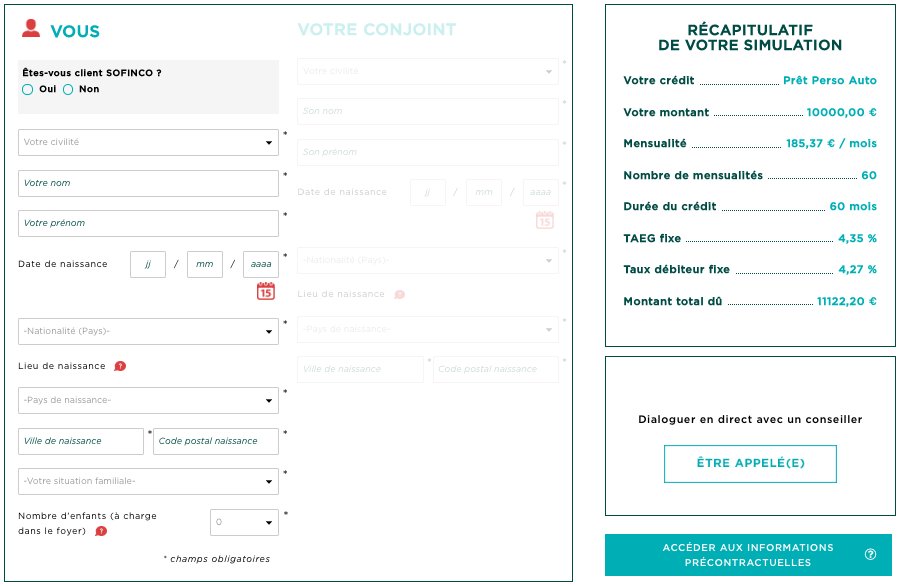
\includegraphics[width=15cm]{figures/chapitre1/souscription.png}
\caption{\label{fig:souscription} Formulaire de souscription d'un crédit automobile Sofinco.}
\end{figure}

% parler des degrés de certitude de l'information

% Montrer l'équivalence formulaire de souscription / alimentation des tables SAS

% Introduire x / données structurées

\subsection{Préparation des données}


% Parler de discrétisation comme d'une technique de gestion des manquants et des outliers + côté pratique et historique

% Sélection de variables basée sur les corrélations et l'expertise métier


\subsection{Critère à modéliser}

% Profitabilité du crédit

% Notion finance -> notion risque

% Temporalité du crédit

% Horizon risque

% Impayés consécutifs

% Passage en pertes

\subsection{Données d'apprentissage}

% Introduire x avec des trous

% Introduire y avec des trous

% Passage aux données complètes par sélection / discrétisation / suppression des non financés

\subsection{L'apprentissage d'une règle de décision}

% Régression logistique (et proc logistic SAS)

% Procédure stepwise

% Calibration des scores

\subsection{La métrique de performance}

% Gini et AUC

% Problèmes à l'utilisation de ces métriques

% Difficultées liées à l'utilisation d'une matrice de confusion

\subsection{Suivi temporel de la performance du score}

% Population drift

% Quand refondre une grille ?

% Un problème qui peut se réinterpréter comme de l'apprentissage par renforcement

\section{Apprentissage statistique} \label{chap1:sec3}


\subsection{Mécanisme de génération des données}


\subsection{Apprentissage semi-supervisé}


\subsection{Apprentissage supervisé}


\subsubsection{Sélection de variables}

% Nombreuse réf. + thèse Vidal

\subsubsection{Variable cible}

% SEME

% Autres références biblio ?

\subsubsection{Choix de modèle}



%%%%%%%%%%%%%%%%%%%%%%%%%%%%%%%%%%%%%%%%%%%%%%%%%%

Ce chapitre a permis .


\printbibliography[heading=subbibliography, title=Références du chapitre 1]